\documentclass[ngerman,11pt,a4paper]{article}

\usepackage[T1]{fontenc}
\usepackage[utf8]{inputenc}

\usepackage[ngerman]{babel}
\usepackage[babel,german=quotes]{csquotes}

\usepackage{graphicx}
\usepackage{babel}
\usepackage{setspace}
%\usepackage{ragged2e}
%\usepackage{float}
%\usepackage{caption}
\usepackage[left=2.5cm, right=2.5cm, top=2.5cm, bottom=2.5cm]{geometry}
%\usepackage{natbib}
\usepackage{amsmath, amsfonts, amssymb}
%\usepackage{cleveref}
%\usepackage{tabto}
%\usepackage{fixltx2e}
%\usepackage{array}
\usepackage{longtable}
%\usepackage{pdflscape}
\usepackage{url}
%\usepackage{subcaption}
\usepackage{siunitx}

\usepackage[style=apa,backend=biber]{biblatex}
\addbibresource{references.bib}

\begin{document}

	\thispagestyle{empty}
	\setstretch{1.5}

	\begin{center}

		\vspace*{1cm}

		\textbf{\huge{Entwicklung einer Universalmethode zur Umsetzung der Wassserrahmenrichtlinie}}

		\vspace{2cm}

		\textbf{\Large{Seminararbeit}}

		\vspace{2cm}

		Technische Universität Dresden\\
		Fakultät Umweltwissenschaften\\
		Institut für Hydrobiologie\\
		Professur für Limnologie (Gewässerökologie)

	\end{center}

	\vspace{4cm}

	\begin{tabbing}
		\hspace{1cm} \= \hspace{4cm} \= \kill

		\> Eingereicht von \> Lisa Wasseramsel\\

    \> Matrikelnummer \> 12345678\\

    \> Studiengang \> Bachelor Hydrowissenschaften\\

		\> Erstprüferin \> Prof. Annegret Clearwater (TU Dresden)\\

		\> Zweitprüfer \> Dr. Michael Fischer (Umweltforschungszentrum)\\

		\> Zeitraum \> 03.06.2024 - 02.09.2024

	\end{tabbing}


	\vspace{4cm}


Dresden, 02.09.2024

\pagebreak

\setstretch{1.2} % normaler Fliesstext 1.2 zeilig

%% ========= Beginn des Hauptteils ===========================================

\section{Einleitung}

Diese Formatvorlage basiert auf einer von einem Studenten beigetragenen Vorlage.
Das Layout basiert auf der Standard-\textbf{article}-Klasse und das Titelblatt
ist mit \verb#vspace#-Befehlen strukturiert. Diese vergleichsweise simple Methode
erlaubt einfache Anpassungen ohne tiefere \LaTeX-Kenntnisse.


\section{Methoden}

\subsection{Untersuchungsgebiet}

Mit bibLaTeX werden aktive Zitate (auch narrativ genannt) mit
\texttt{\textbackslash cite\{\}}: \cite{r-core-2024} und passive Zitate (auch
eingeklammert genannt) mit \texttt{\textbackslash parencite\{\}} gesetzt:
\parencite{r-core-2024}.

\subsection{Gewässerbewertung}

\subsubsection{Vor-Ort-Verfahren}

\subsubsection{Auswertung von Satellitendaten}

\subsubsection{Berechnungen}

Mathemathische Gleichungen und Formeln können mit der \texttt{equation}-Umgebung
gesetzt werden:

\begin{equation}
	y = \alpha + \beta \cdot x + \epsilon
\end{equation}

Für Gleichungen mit mehreren Zeilen eignet sich die \texttt{align} Umgebung gut,
bei der man z.B. das Gleichheitszeichen untereinander ausrichten kann.

\begin{align}
\frac{dP}{dt} &= r \cdot f(S) \cdot P \\
\frac{dS}{dt} &= - \frac{1}{Y} \cdot P \\
f(S) &= r_{max} \cdot \frac{S}{k_S + S}
\end{align}

Für Maßeinheiten und chemische Formeln existieren unterschiedliche Methoden.
Einfach und pragmatisch ist die Kombination aus Mathematikmodus (mit \verb#$$#)
und \verb#mathrm{}#, damit die Maßeinheiten nicht kursiv gesetzt werden.


Code: \verb#$\mathrm{\mu g L^{-1}}$, $\mathrm{PO_4^{3-}}$#

Ergebnis: $\mathrm{\mu g L^{-1}}$, $\mathrm{PO_4^{3-}}$

Das funktioniert soweit, gilt aber typografisch als nicht ganz sauber.
Stattdessen werden die Pakete \textbf{siunitx} und \textbf{mchem} empfohlen.


\subsection{Statistische Analyse}

Die statistische Analyse wurde mit \textbf{R} \parencite{r-core-2024} und RStudio
\parencite{rstudio-2024} durchgeführt. Für die Grafiken
wurde das Paket \textbf{ggplot2} verwendet \parencite{wickham-ggplot2-2016}.


\section{Ergebnisse}

Lorem ipsum dolor sit amet, consetetur sadipscing elitr, sed diam nonumy eirmod
tempor invidunt ut labore et dolore magna aliquyam erat, sed diam voluptua. At
vero eos et accusam et justo duo dolores et ea rebum. Stet clita kasd gubergren,
no sea takimata sanctus est Lorem ipsum dolor sit amet. Lorem ipsum dolor sit
amet, consetetur sadipscing elitr, sed diam nonumy eirmod tempor invidunt ut
labore et dolore magna aliquyam erat, sed diam voluptua. At vero eos et accusam
et justo duo dolores et ea rebum. Stet clita kasd gubergren, no sea takimata
sanctus est Lorem ipsum dolor sit amet (siehe Abbildung \ref{fig:fig_1}).

Test von Umlauten und Sonderzeichen äöü ÄÖÜ ßßß µ @ €. Dieser Test soll zeigen,
ob die Schriftarten richtig funktionieren, wenn der Text im UTF-8-Format
abgespeichert wurde.


\begin{figure}
	\centering
	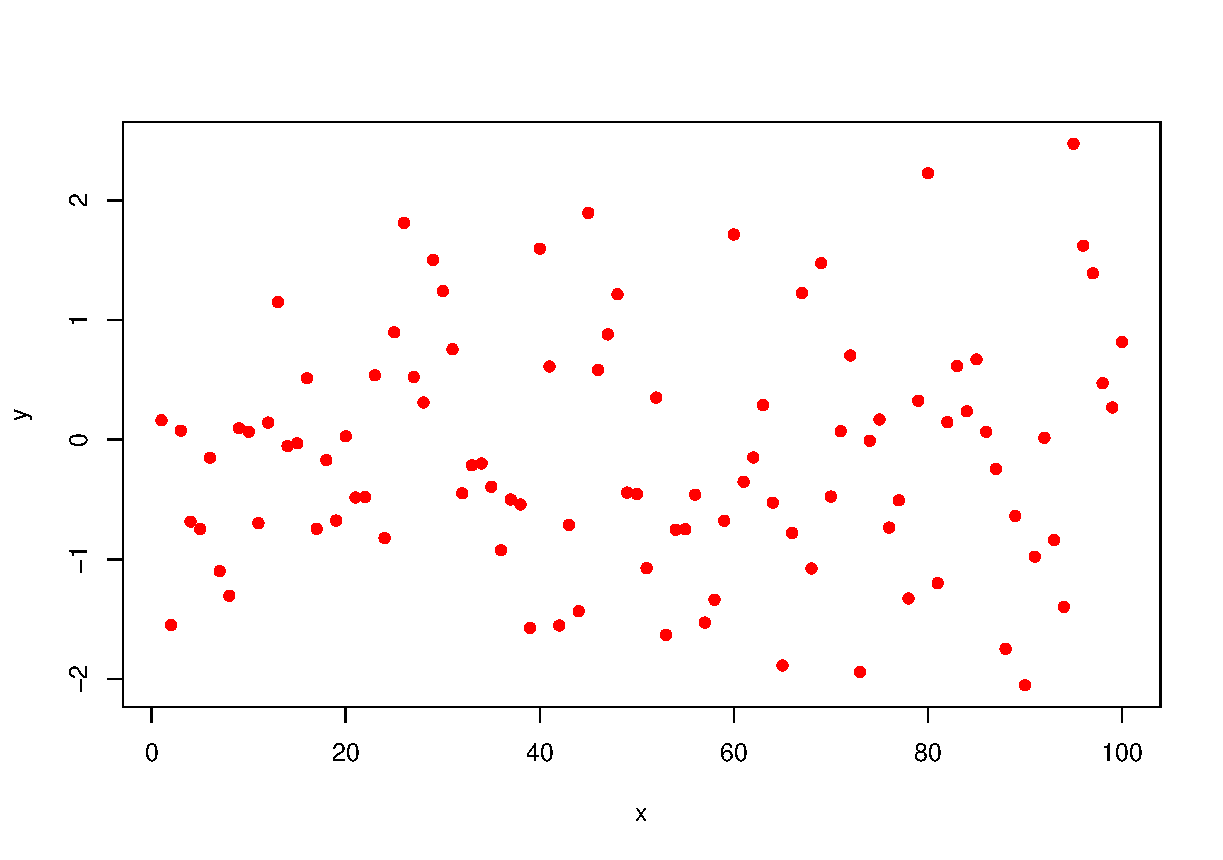
\includegraphics[width=\textwidth]{pdf-plot.pdf}
	\caption[Kurzfassung des Abbildungstitels]{Langfassung des Abbildungstitels,
	         meistens 2-5 Zeilen}\label{fig:fig_1}
\end{figure}

\begin{table}
	\centering
	\caption[Kurzfassung der Tabellenüberschrft]{Langfassung der Tabellenüberschrift,
	        im Regelfall mehrere Zeilen. Es sollten insbesondere Abkürzungen erklärt werden.}
	\label{tab:my_label}
	\begin{tabular}{lll}\hline
		Name & Probenahmestelle & Wert\\\hline
		Temperatur & 1  & 14  \\
		Sauerstof & 2  & 16 \\
		Trübung & 3 & 15 \\ \hline
	\end{tabular}
\end{table}


\section{Diskussion}

Hier werden die Aufgaben und Hypothesen aus der Einleitung aufgegriffen und
argumentativ untersetzt. Potentielle Defizite und Fehler werden eingeräumt und
eingeordnet. Es sollte das Positive herausgearbeitet werden, außer wenn alles
schief gegangen ist, was selten der Fall ist.

\section*{Danksagung} % \section*{} erzeugt keine Nummerierung für das Kapitel und keinen Eintrag im Inhaltsverzeichnis
\addcontentsline{toc}{chapter}{Danksagung} % Ergänzt die Danksagung im Inhaltsverzeichnis


Die Danksagung kann individuell gestaltet werden. Wichtig ist vor allem,
Praxispartnern zu danken und den Leuten oder Organisationen, von denen man
finanziellen Support oder Daten bekommen hat. Bei BMBF-, DFG-, EU- und anderen
Projekten ist die Nennung des Förderkennzeichens in den Förderrichtlinien
vorgeschrieben.

\section*{Selbständigkeitserklärung}
\addcontentsline{toc}{chapter}{Selbständigkeitserklärung}

Bei Prüfungs und Abschlussarbeiten muss im Regelfall eine Selbständigkeitserklärung angegeben werden.



\printbibliography


% Falls ein Anhang gewünscht ist kann dieser hier ergänzt werden. Die Kapitelnummerierung wird für
% den Anhang auf Buchstaben geändert

\setcounter{section}{0}
\renewcommand\thesection{\Alph{section}}
\section{Ergänzende Grafiken}

Falls ein Anhang nötig ist kann dieser hier ergänzt werden

\begin{figure}[h]
	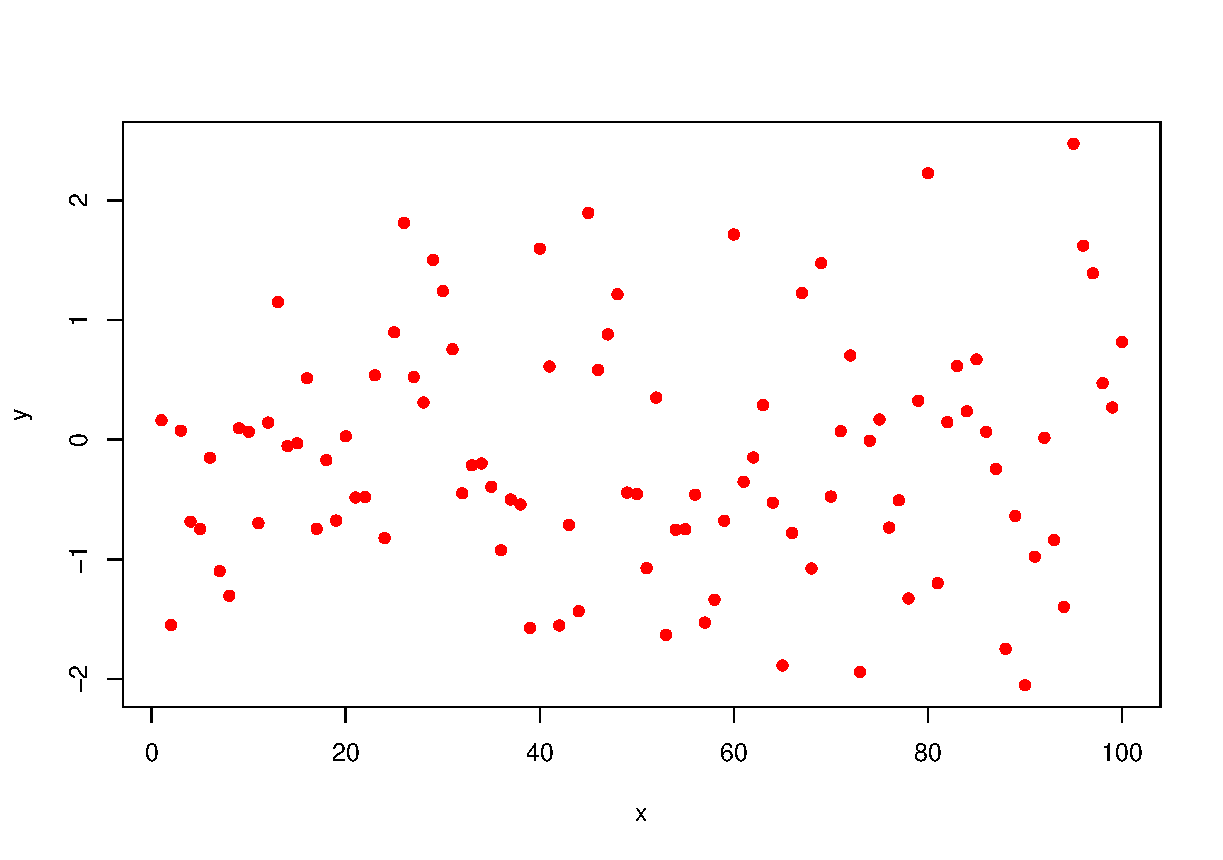
\includegraphics[width=\linewidth]{pdf-plot.pdf}
	\caption[kurze Beschreibung für die Liste der Abbildungen]{Lange Beschreibung für den Fließtext}
\end{figure}


\end{document}
